
\subsection{The Server}
An API server was written in python, as due to the small scale of the application, this was ideal to meet the requirements whilst keeping the 
implementation simple enough. The server provides several endpoints which may be pinged, but only two particular endpoints are used. 
\subsubsection{Location Updates}
The server keeps track of a list of active devices, (though a unique identifier provided on requests), and their last known location.
The device regularly updates the sever with location information, and then requests nearby landmark data. 
The server loops through all landmarks, and calculates the distance between the device longitude and latitude positioning, and the landmark.
If the distance is below some threshold, it is added to a list of potentially explorable landmarks, which is returned as a JSON response 
to the device. Each landmark entry also contains a geofence region, which when is larger than the distance, the landmarks are considered near 
the user, and the device can know that the AR mode can be enabled.


\subsection{Landmark Menu}
\subsubsection{General User Interface}
Unity provides a wide range of features that can be used to implemented UI in the application. 
Modern solutions make use of a canvas gameObject which promises several features such as user interaction, screen scaling/responsiveness, and 
list managing features such as scrollable lists.
\noindent
A scrollable list was used to show a list of the landmarks returned by the server. The title,
a short description, the raw distance from the location and the bearing to the location is shown for each entry,
 so the user may have some basic information on how to reach a target.
  Whenever some landmark is very close, the entry becomes interactable, and the user can press it 
to enter AR mode near the landmark. 

\subsubsection{Location Service}
On the device, the location is updated every second, with an intended accuracy of 0.1 metres 
(usually not met, but we try to be as accurate as possible).\\
The integrated unity function is used, and a listener is used to check for updates, which update the server,
and the landmarks list accordingly.


% \subsubsection{Geometric }
\subsubsection{Geometric Bearing, Distance \& Geofencing}
In the aims of ensuring timely server responses, a library called 'haversine' was used to calculate distances between two coordinates. This is not very straightforward, 
as in calculations one needs to consider the curvature of the earth, and take distance measurements as lengths in circumference. Each landmarks entry has a "rad" 
attribute, and when the distance between the device and landmarks is smaller, the device can be considered as being inside the geofence!\\
The Geometric bearing was calculated on the device, as the server did not have many other uses for the bearing of the device. Here we once again use the coordinates 
of the device, the current magnetic heading of the device and the coordinates of the landmark to find a relative bearing (clockwise angle from the north).   

% \subusbsection{Geometric Bearing}


% \subsection{Main Techniques}
% The main algorithms used deal with the positioning and distance calculations of the device.

\subsection{AR Mode Technologies}
In this mode, the camera is shown to the user, and a 3D translucent floating window is spawned in 3D space.
The user may move around the panel, and observe the panel stays locked in 3D space. The panel shows
some deeper description of the near landmark. A carousel allows the user to see some images of the place
 (as provided through the API). 

% \subsection{Scaling}


\subsubsection{Fixed Positioning \& Interactability}
When combined with unity, ARCore gives the developer access to the AR camera and the pose driver, which are responsible for synchronizing movements 
carried out in real life, with the movement inside the game engine. A 'World Canvas' gameObject was used so that we can use UI features in 3D space, allowing for a simpler implementation when 
handling image placement, text sizing, and any other form of user interaction with the panel. By appending the information panel to this type of canvas, we also inform ARCore that 
we want to synchronise the gameObject positioning between the real world and the virtual unity world space.\\
\noindent
Through the aforementioned pose driver and AR camera, a system is used where 1 unit in the unity engine corresponds to 1 meter when
viewed in AR mode. Thus If we need to create a 30cm box, we can just set the size in the engine to 0.3, without needing to do any manual conversion, etc.
% \subsubsection{Scaling}

\subsubsection{Information Panel Instantiation}
Using the aforementioned techniques, we first create a generic prefab for the Information Panel. This includes the colouring, text placement, title placement, and 
other things such as button placement and functionality etc. We also provide some relative sizing, which will be scaled accordingly when the prefab is used.\\ 
The Instantiation of the information panel happens upon clicking on the desired entry from the landmarks menu, where the information of the landmark is transferred to the AR Mode scene.
This information includes data such as the landmark title, a long description and an array of image URLs. We then simply populate the prefab with the information provided and instantiate 
the panel as a child of the world canvas, relative to the AR camera position. 
The Pose driver then ensures that the panel stays fixed in the in-game position, whilst varying the AR camera position to 
match real-world movements of the device. 



%  \subsection{Other AR Techniques}
%  A couple of other Augmented Reality techniques were explored during the development of this app. 
%  These techniques were implemented and worked well as stand-alone, yet when combining the features, 
%  these standalone techniques were omitted, as they would require infrastructural changes to the way that landmarks are stored and communicated, which I believe is out of the scope for this project. They are still left available in the unity project in case these would be implemented in the future yet as is, there is no way of accessing them through the App. 
%  \subsubsection{Plane detection}
%  Although raw plane detection was not used in the final version, under the hood google uses it to keep the 
%  floating information panel in place. Through goggle's AR Core it is made possible to detect vertical 
%  and horizontal planes, to which other game objects can be anchored to!\\

%  In an example, plane detection was used to find a stable surface, and when the user clicks on a 
%  plane, a 3D Game model is spawned in place and anchored to the plane. The user is also able to walk around 
%  in the room, whilst the objects stay anchored to the plane! 

%  \subsection{Image Recognition \& Augmented Images}
%  Image Recognition was also a really interesting feature to use, yet unfortunately, it is not used in the application. This may have been able to be implemented, yet with the current implementations 
%  of the landmark menu and the ARMode switching, It did not make much sense to be used. (As in the near landmark menu, there is no access to the camera), and the user may only use AR Mode when near a landmark.\\
%  However, this feature is also fully working, and may easily be implemented if a better use in the context of outdoor AR is identified. 
%  In the case of this project, a quick database manager was created in which a list of images could
%   be inserted. These images also need to have specific features, to be distinguishable from other places (for example some image of plain grey gravel is not very easily distinguishable, 
%   but an image of the earth is). And actions would be taken according to the image detected!
\subsection{Testing Performed}
Due to the domain of this project and the technologies adopted, it was not as straightforward to 
test the raw performance of the system. As there is no performance metric or such that can be 
analysed and compares to other instances \cite{Samini2017}. 
\subsubsection{On-Site Testing}
Several tests were performed on-site, where the locations were actually based, all with the aims of exploring how the system handles different cases. 
This included normal usability and even edge cases such as using the panel where we know plane detection will struggle.
\\
Firstly, the panel was tested on floors that had discernable planes features, and on others where there was a repeated pattern (a known struggle-point of plane detection).\\
\begin{figure}[!htb]
    \minipage{0.32\textwidth}
        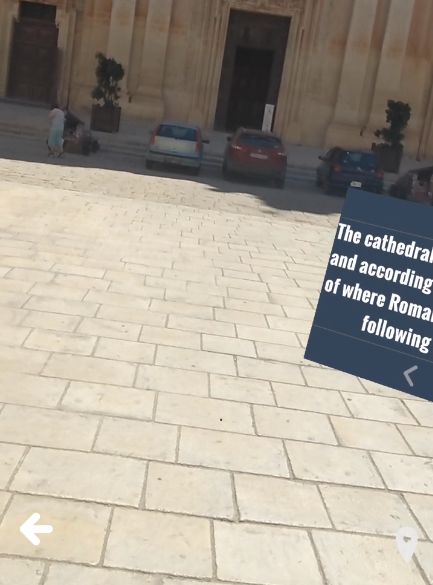
\includegraphics[width=\linewidth]{bad_floor_panel_glitch}
            \caption{Panel Glitching due to repeated pattern}
            \label{fig:bad_panel}
    \endminipage\hfill
    \minipage{0.32\textwidth}
        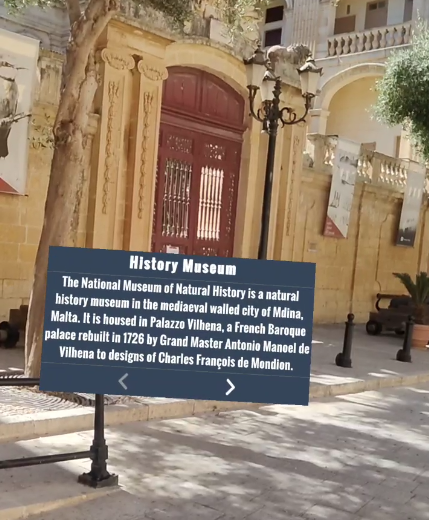
\includegraphics[width=\linewidth]{history_museum_text_panel}
        \caption{Stable Panel showing text}
        \label{fig:panel_text}
    \endminipage\hfill
    \minipage{0.32\textwidth}%
        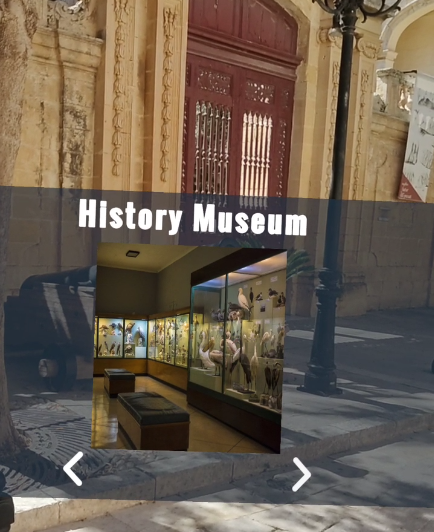
\includegraphics[width=\linewidth]{history_museum_image_panel1}
        \caption{Stable Panel showing image}
        \label{fig:panel_img}
    \endminipage
    \end{figure}

\noindent
Figures \ref{fig:bad_panel}, \ref{fig:panel_text} and \ref{fig:panel_img}
show the panels in action on the different conditions tested. As can be seen, in good conditions, the panels stay in place 
and are also interactable, where one can see text and the carousel of images, behaving as expected.
Next, in order to test the bearing accuracy, the north pole was temporarily added as a landmark, and a general comparison between the bearing shown and a compass was used.
The application was also used with a subpar GPS connection to see the impact on the overall experience (as some parts of Mdina do not have good coverage).

\begin{figure}[!htb]
    \minipage{0.45\textwidth}
        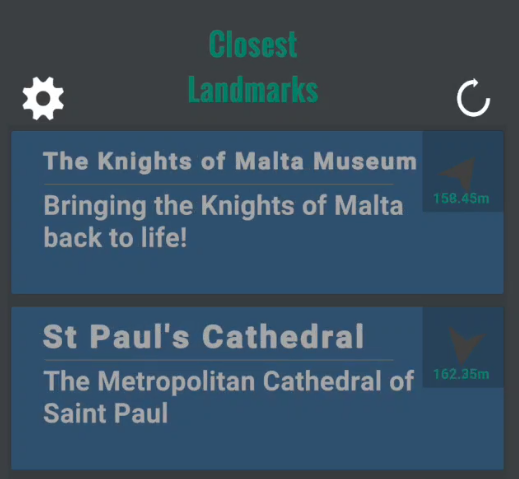
\includegraphics[width=\linewidth]{landmarks_menu}
            \caption{Explorable Landmark Entries}
            \label{fig:explor_lands}
    \endminipage\hfill
    \minipage{0.45\textwidth}
        
\includegraphics[width=\linewidth]{landmarks_menu_activated}
        \caption{Landmark Entry Activated (In geofence)}
        \label{fig:active_land}
    \endminipage
    \end{figure}
\noindent
Finally, Figures \ref{fig:explor_lands} and \ref{fig:active_land} show the landmarks menu, both 
when the user is not inside the geofence and also how the UI changes when the user is inside.\\
Further testing is shown in the video, as it's the best way to convey the experience.
